%%%%%%%%%%%%%%%%%%%%%%%%%%%

\chapter{Characterization of magnetic contamination}\label{appx:magnetic_contamination}

%%%%%%%%%%%%%%%%%%%%%%%%%%%

Magnetic impurities detected by the scanner (Sec.~\ref{sec:magnetic_impurity_scanner}) to first order may be treated as a dipole. In this appendix we describe the method used to determine the magnetic moment $\vv{m}$ of such a dipole. The magnetic field produced by a dipole is given by \cite{chow2006introduction}
%
\begin{gather}
    \vv{B}_m({\vv{r}}) = \frac{\mu_{0}}{4\pi}\left(\frac{3\vv{r}(\vv{m}\cdot\vv{r})}{r^{5}} - \frac{{\vv{m}}}{r^{3}}\right)
\end{gather}

The magnetic field falls off $\propto 1/r^3$, which we use to determine the distance between the magnetometers and the dipole. This approach was adopted to account for a common source of magnetic contamination, threaded holes tapped with previously-used tooling. (This led to a specification to vendors to use a designated set of tooling only for the LANL nEDM.) Because contamination could be buried deep within the threaded hole, a measurement of the distance between the magnetometers and the start of the hole was insufficient.

Let $B_\text{low}(r)$ be the field read by the magnetometer closer to dipole and $B_\text{up}(r)$ be the field read by the further one. When the contamination on the turntable is directly beneath the magnetometers ($r=r_\text{min}$), we write the expression
%
\begin{gather}
    B_\text{up}(r_\text{min})\,(r_\text{min} + x_\text{sep})^3 = B_\text{low}(r_\text{min})\,(r_\text{min})^3 \label{eq:magnetic_contamination_1}
\end{gather}
%
where $x_\text{sep}=\qty{0.75}{in}=\qty{0.01905}{m}$ is the separation between the magnetometers.

Using the data from Fig.~\ref{fig:magnetic_contamination_example} as an example, we solve Eq.~(\ref{eq:magnetic_contamination_1}) for $r_\text{min}$ each time the dipole passes beneath the magnetometers. This gives $r_\text{min}=\qty{0.024(5)}{m}$ where the error is given by the standard deviation.

The x-axis (time) of Fig.~\ref{fig:magnetic_contamination_example} was converted to turntable angle $\theta$ using the radial location of the magnetometers relative to the center of the turntable ($\qty{0.2}{m}$) and the turntable period of rotation ($\sim\qty{48}{s}$). Background drift was also approximated by a linear regression fit using the data at the beginning and the end of the run. The data was then fit to
%
\begin{gather}
    \vv{B}_m({\vv{r}}) + B_\text{offset}\label{eq:dipole_fitting}
\end{gather}
%
where $B_\text{offset}$ is a free parameter to account for the baseline magnetic field read by the magnetometer.

Results are shown in Fig.~\ref{fig:lower_quspin_contamination_fit}. For simplicity $\vv{m}$ was oriented along the vector of the dipole's velocity when it was beneath the magnetometers. This gave a fit result of $m=\qty{80.9(7)e-9}{A\,m^2}$, $B_\text{offset}=\qty{0.042(4)e-9}{T}$, and $\text{Corr}(m, B_\text{offset})=-0.9$.

\comment{Update with Lilian's work as quantification of current loop on a turntable continues}

\begin{figure}
    \centering
    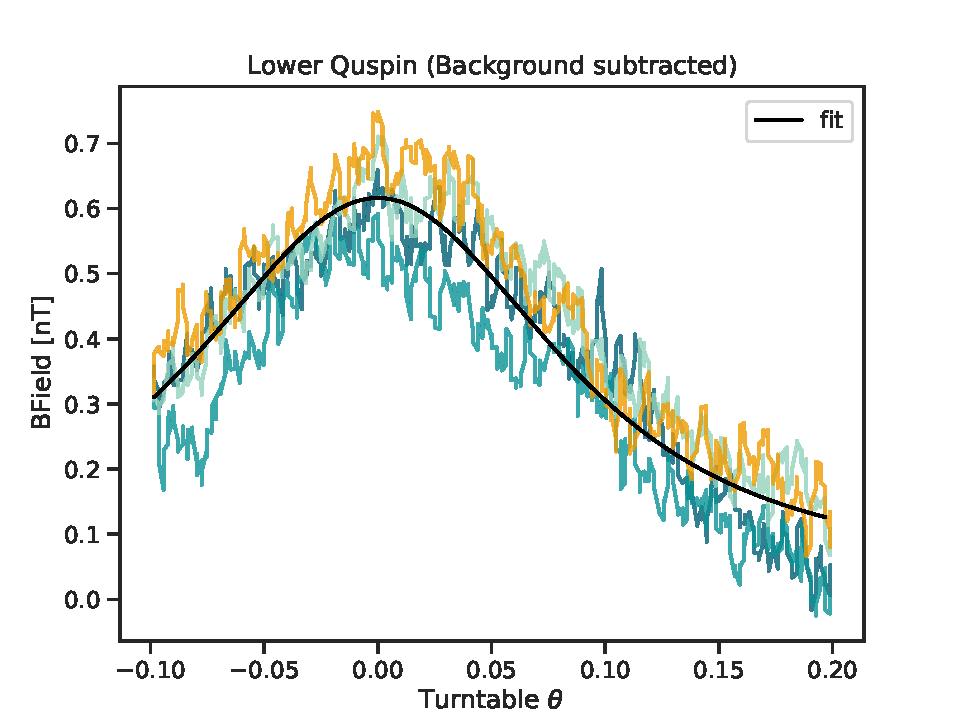
\includegraphics[width=0.7 \textwidth]{figures/quspin_fit.pdf}
    \caption
    {Fit of Eq.~\ref{eq:dipole_fitting} to data from Fig.~\ref{fig:magnetic_contamination_example}}
    \label{fig:lower_quspin_contamination_fit}
\end{figure}